% ****** Start of file apssamp.tex ******
%
%   This file is part of the APS files in the REVTeX 4.2 distribution.
%   Version 4.2a of REVTeX, December 2014
%
%   Copyright (c) 2014 The American Physical Society.
%
%   See the REVTeX 4 README file for restrictions and more information.
%
% TeX'ing this file requires that you have AMS-LaTeX 2.0 installed
% as well as the rest of the prerequisites for REVTeX 4.2
%
% See the REVTeX 4 README file
% It also requires running BibTeX. The commands are as follows:
%
%  1)  latex apssamp.tex
%  2)  bibtex apssamp
%  3)  latex apssamp.tex
%  4)  latex apssamp.tex
%
\documentclass[%
 reprint,
%superscriptaddress,
%groupedaddress,
%unsortedaddress,
%runinaddress,
%frontmatterverbose, 
%preprint,
%preprintnumbers,
%nofootinbib,
%nobibnotes,
%bibnotes,
 amsmath,amssymb,
 aps,
%pra,
%prb,
%rmp,
%prstab,
%prstper,
%floatfix,
]{revtex4-2}
\usepackage{multirow}
\usepackage{graphicx}% Include figure files
\usepackage{dcolumn}% Align table columns on decimal point
\usepackage{bm}% bold math
%\usepackage{hyperref}% add hypertext capabilities
%\usepackage[mathlines]{lineno}% Enable numbering of text and display math
%\linenumbers\relax % Commence numbering lines

%\usepackage[showframe,%Uncomment any one of the following lines to test 
%%scale=0.7, marginratio={1:1, 2:3}, ignoreall,% default settings
%%text={7in,10in},centering,
%%margin=1.5in,
%%total={6.5in,8.75in}, top=1.2in, left=0.9in, includefoot,
%%height=10in,a5paper,hmargin={3cm,0.8in},
%]{geometry}
\usepackage[utf8x]{inputenc} % Включаем поддержку UTF8  
\usepackage[russian]{babel}  % Включаем пакет для поддержки русского языка 
\usepackage[normalem]{ulem}  % для зачекивания текста


\usepackage[noend]{algorithmic}
\def\algorithmicrequire{\textbf{Вход:}}
\def\algorithmicensure{\textbf{Выход:}}
\def\algorithmicif{\textbf{если}}
\def\algorithmicthen{\textbf{то}}
\def\algorithmicelse{\textbf{иначе}}
\def\algorithmicelsif{\textbf{иначе если}}
\def\algorithmicfor{\textbf{для}}
\def\algorithmicforall{\textbf{для всех}}
\def\algorithmicdo{}
\def\algorithmicwhile{\textbf{пока}}
\def\algorithmicrepeat{\textbf{повторять}}
\def\algorithmicuntil{\textbf{пока}}
\def\algorithmicloop{\textbf{цикл}}
% переопределение стиля комментариев
\def\algorithmiccomment#1{\quad// {\sl #1}}

\begin{document}



\title{Лабораторная работа 5.5\\Компьютерная сцинтилляционная $\gamma$-спектропия}% Force line breaks with \\



\author{Батарин Егор Владиславович}
\affiliation{%
 Студент 3 курса РТ\\
}%

\collaboration{Московский физико-технический институт}%\noaffiliation

\date{6 сентября 2021 г.}% It is always \today, today,
             %  but any date may be explicitly specified
             

\begin{abstract}
Определяется энергия $\gamma$ - квантов неизвестного радиактивного препарата, определяется энергетическое разрешение спектрометра для разных образцов, а также энергия излучаемого характеристического излучения свинца по спектральному графику.
\begin{description}
\item[Оборудование]
Компьютер, сцинтиллятор, 5 образцов с радиоактивными материалами.
\end{description}
\end{abstract}

%\keywords{Suggested keywords}%Use showkeys class option if keyword
                              %display desired
\maketitle

%\tableofcontents

\section{Теоретическая часть.}
\subsection{Введение в основные эффекты лабы.}


Основными процессами взаимодействия гамма-излучения с веществом
являются фотоэффект, эффект Комптона и образование электрон-позитронных пар. Каждый из этих процессов вносит свой вклад в образование наблюдаемого спектра. 

\textbf{Фотоэффект} - процесс взаимодействия гамма-кванта с электроном, связанным с атомом, 
при котором электрону передается вся энергия гамма-кванта.

\textbf{Эффект Комптона} – упругое рассеяние фотона на свободном электроне,
сопровождающееся изменением длины волны фотона (реально этот процесс
происходит на слабо связанных с атомом внешних электронах). 

\textbf{Процесс образования электрон-позитронных пар.} При достаточно высокой энергии гамма-кванта наряду с фотоэффектом и эффектом Комптона
может происходить третий вид взаимодействия гамма-квантов с веществом –
образование электрон-позитронных пар. 

\subsection{Физика процессов, лежащих в основе эксперимента.}

Принцип действия сцинтиллятора можно разбить на несколько шагов:

1) Гамма-кванты от исследуемого объекта попадают в сцинтиллятор NaI(Tl).

2) Они взаимодействуют с веществом и вырывают электроны из атомных оболочек (конверсионные электроны).

3) Конверсионные электроны тормозятся в сцинтилляторе, передавая свою энергию атомам NaI(Tl).

4) Возбужденные атомы излучают фотоны (видимый и ультрафиолетовый спектр).

5) Часть этих фотонов, пройдя через сцинтиллятор, попадает на катод ФЭУ, выбивая из него медленные электроны.

6) Эти электроны ускоряются электрическим полем умножителя, и попав на поверхность первого динода, вырывают из него электроны, которые в свою очередь попадают на поверхность второго динода, и т.д. 

7) Образовавшаяся лавина электронов формируется и записывается в память компьютера.

Можно подобрать напряжения на динодах ФЭУ так, чтобы величина выходного импульса, фиксируемого компьютером, была пропорциональна числу фотонов на шаге 5. Число этих фотонов, в свою очередь, пропорционально энергии конверсионных электронов, а их энергия пропорциональна энергии первичных гамма-квантов. Эта цепочка пропорциональностей дает возможность оценивать энергию гамма-квантов изучаемого объекта по выходным импульсам, анализируемым на компьютере. 

\subsection{Энергетическое разрешение спектрометра.}
Даже при поглощении часна выходе фотоприёмника
сцинтилляционного детектора меняется от события к событию. Это связано:

1) со статистическим характером процессов сбора фотонов на фотоприемнике и последующего усиления.

2) с различной вероятностью доставки фотона к фотоприёмнику из различных точке сцинтиллятора.

Поэтому, графики спектрограмм имеют стохастический характер, а число импульсов является дискретной случайной величиной. Далее, будем применять аппарат теории вероятностей.

Энергетическим разрешением спектрометра называется величина

\begin{equation}
R_i = \frac{\Delta E_i}{E_i}
\end{equation}

где $\Delta E_i$ – ширина пика полного поглощения, измеренная на половине вы-
соты, $E_i$ – энергия регистрируемого гамма-излучения. Значение $E_i$ пропорцио-
нально среднему числу фотонов $n_i$ на выходе ФЭУ, т.е.:
\begin{equation}
E_i = \alpha\overline{n_i}
\end{equation}
Полуширина пика полного поглощения $\Delta E_i$ пропорциональна среднеквадратичной флуктуации $\overline{\Delta n_i}$. Так как $n_i$ - дискретная случайная величина, то  $\overline{\Delta n_i} = \sqrt{\overline{n_i}}$, значит 
\begin{equation}
\Delta E_i = \alpha\overline{\Delta n_i} = \alpha\sqrt{\overline{n_i}}	
\end{equation}

Из этих формул получаем:
\begin{equation}
R_i = \frac{\Delta E_i}{E_i} = \frac{\text{const}}{\sqrt{E_i}}
\end{equation}


\section{Экспериментальная установка и методика}
\subsection{Схема установки.}

Принципиальная блок-схема гамма-спектрометра, изучаемого в данной
работе, показана на рисунке.

\begin{figure}[h!]
	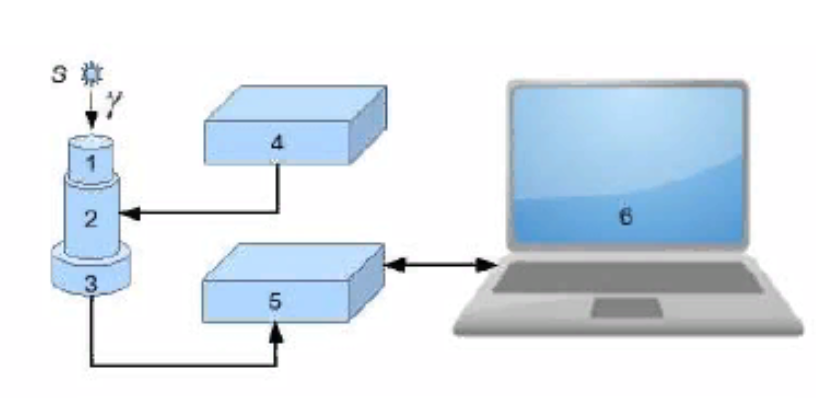
\includegraphics[scale=0.42]{1.png}
\end{figure}


На этом рисунке: 1 – сцинтиллятор, 2 – ФЭУ, 3 – предусилитель импуль-
сов,
4 – высоковольтный блок питания для ФЭУ, 5 – блок преобразования
аналоговых импульсов с ФЭУ в цифровой код (АЦП), 6 – компьютер для
сбора данных, их обработки и хранения.
ФЭУ со сцинтиллятором и блоком питания установлены на отдельной
подставке. В нашей работе на разных установках (стендах) в качестве сцин-
тиллятора используются кристаллы NaI(Tl) с размерами 45x50 мм и 
20x25 мм.
\subsection{Методика работы.}

\begin{algorithmic}[1]
	\REQUIRE 5 образцов радиоактивных элементов;
	\ENSURE записи графиков в компьютере;
	\FORALL{5 образцов}
	\REPEAT
	\STATE берем образец;
	\STATE кладем в сцинтиллятор;
	\STATE запускаем счет импульсов на несколько минут;
	\STATE останавливаем и конвертируем полученные данные в таблицу Excel;
	\UNTIL{образцы не закончатся};	
	\ENDFOR
\end{algorithmic}


\section{Результаты работы и их обсуждение.}

Прежде всего, исследуем, как "ползет" график в зависимости от ручки потенциометра:

\begin{figure}[h!]
	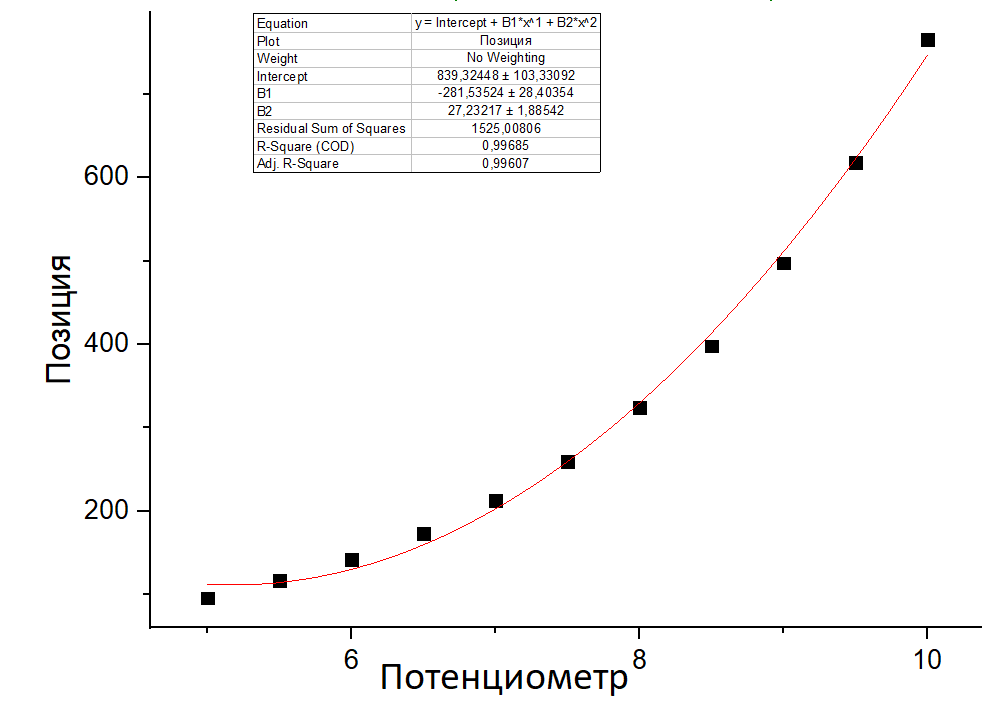
\includegraphics[scale=0.45]{2.png}
\end{figure}

Как видим, смещение графика в зависимости от поворота ручки потенциометра хорошо аппоксимируется квадратичной функцией. Самое маленькое значение потенциометра, на которое он был установлен, среди всех 5 образцов, равно $5.2$ - относительно этого значения будем проводить калибровку. В результате получаем таблицу:

\begin{table}[h!]
	\begin{tabular}{|l|l|l|}
		\hline
		Позиция & Значение кв. функции & Калибровка \\ \hline
		5,2     & 114                  & 0          \\ \hline
		5,4     & 115                  & 1          \\ \hline
		6,3     & 148                  & 34         \\ \hline
		9,5     & 617                  & 503        \\ \hline
		10      & 740                  & 626        \\ \hline
	\end{tabular}
\end{table}


Построим зависимость числа отсчетов $N$ от энергии $E$ и 4 дифференциальные кривые распределения энергии. Получаем:

=

\begin{figure*}[]
	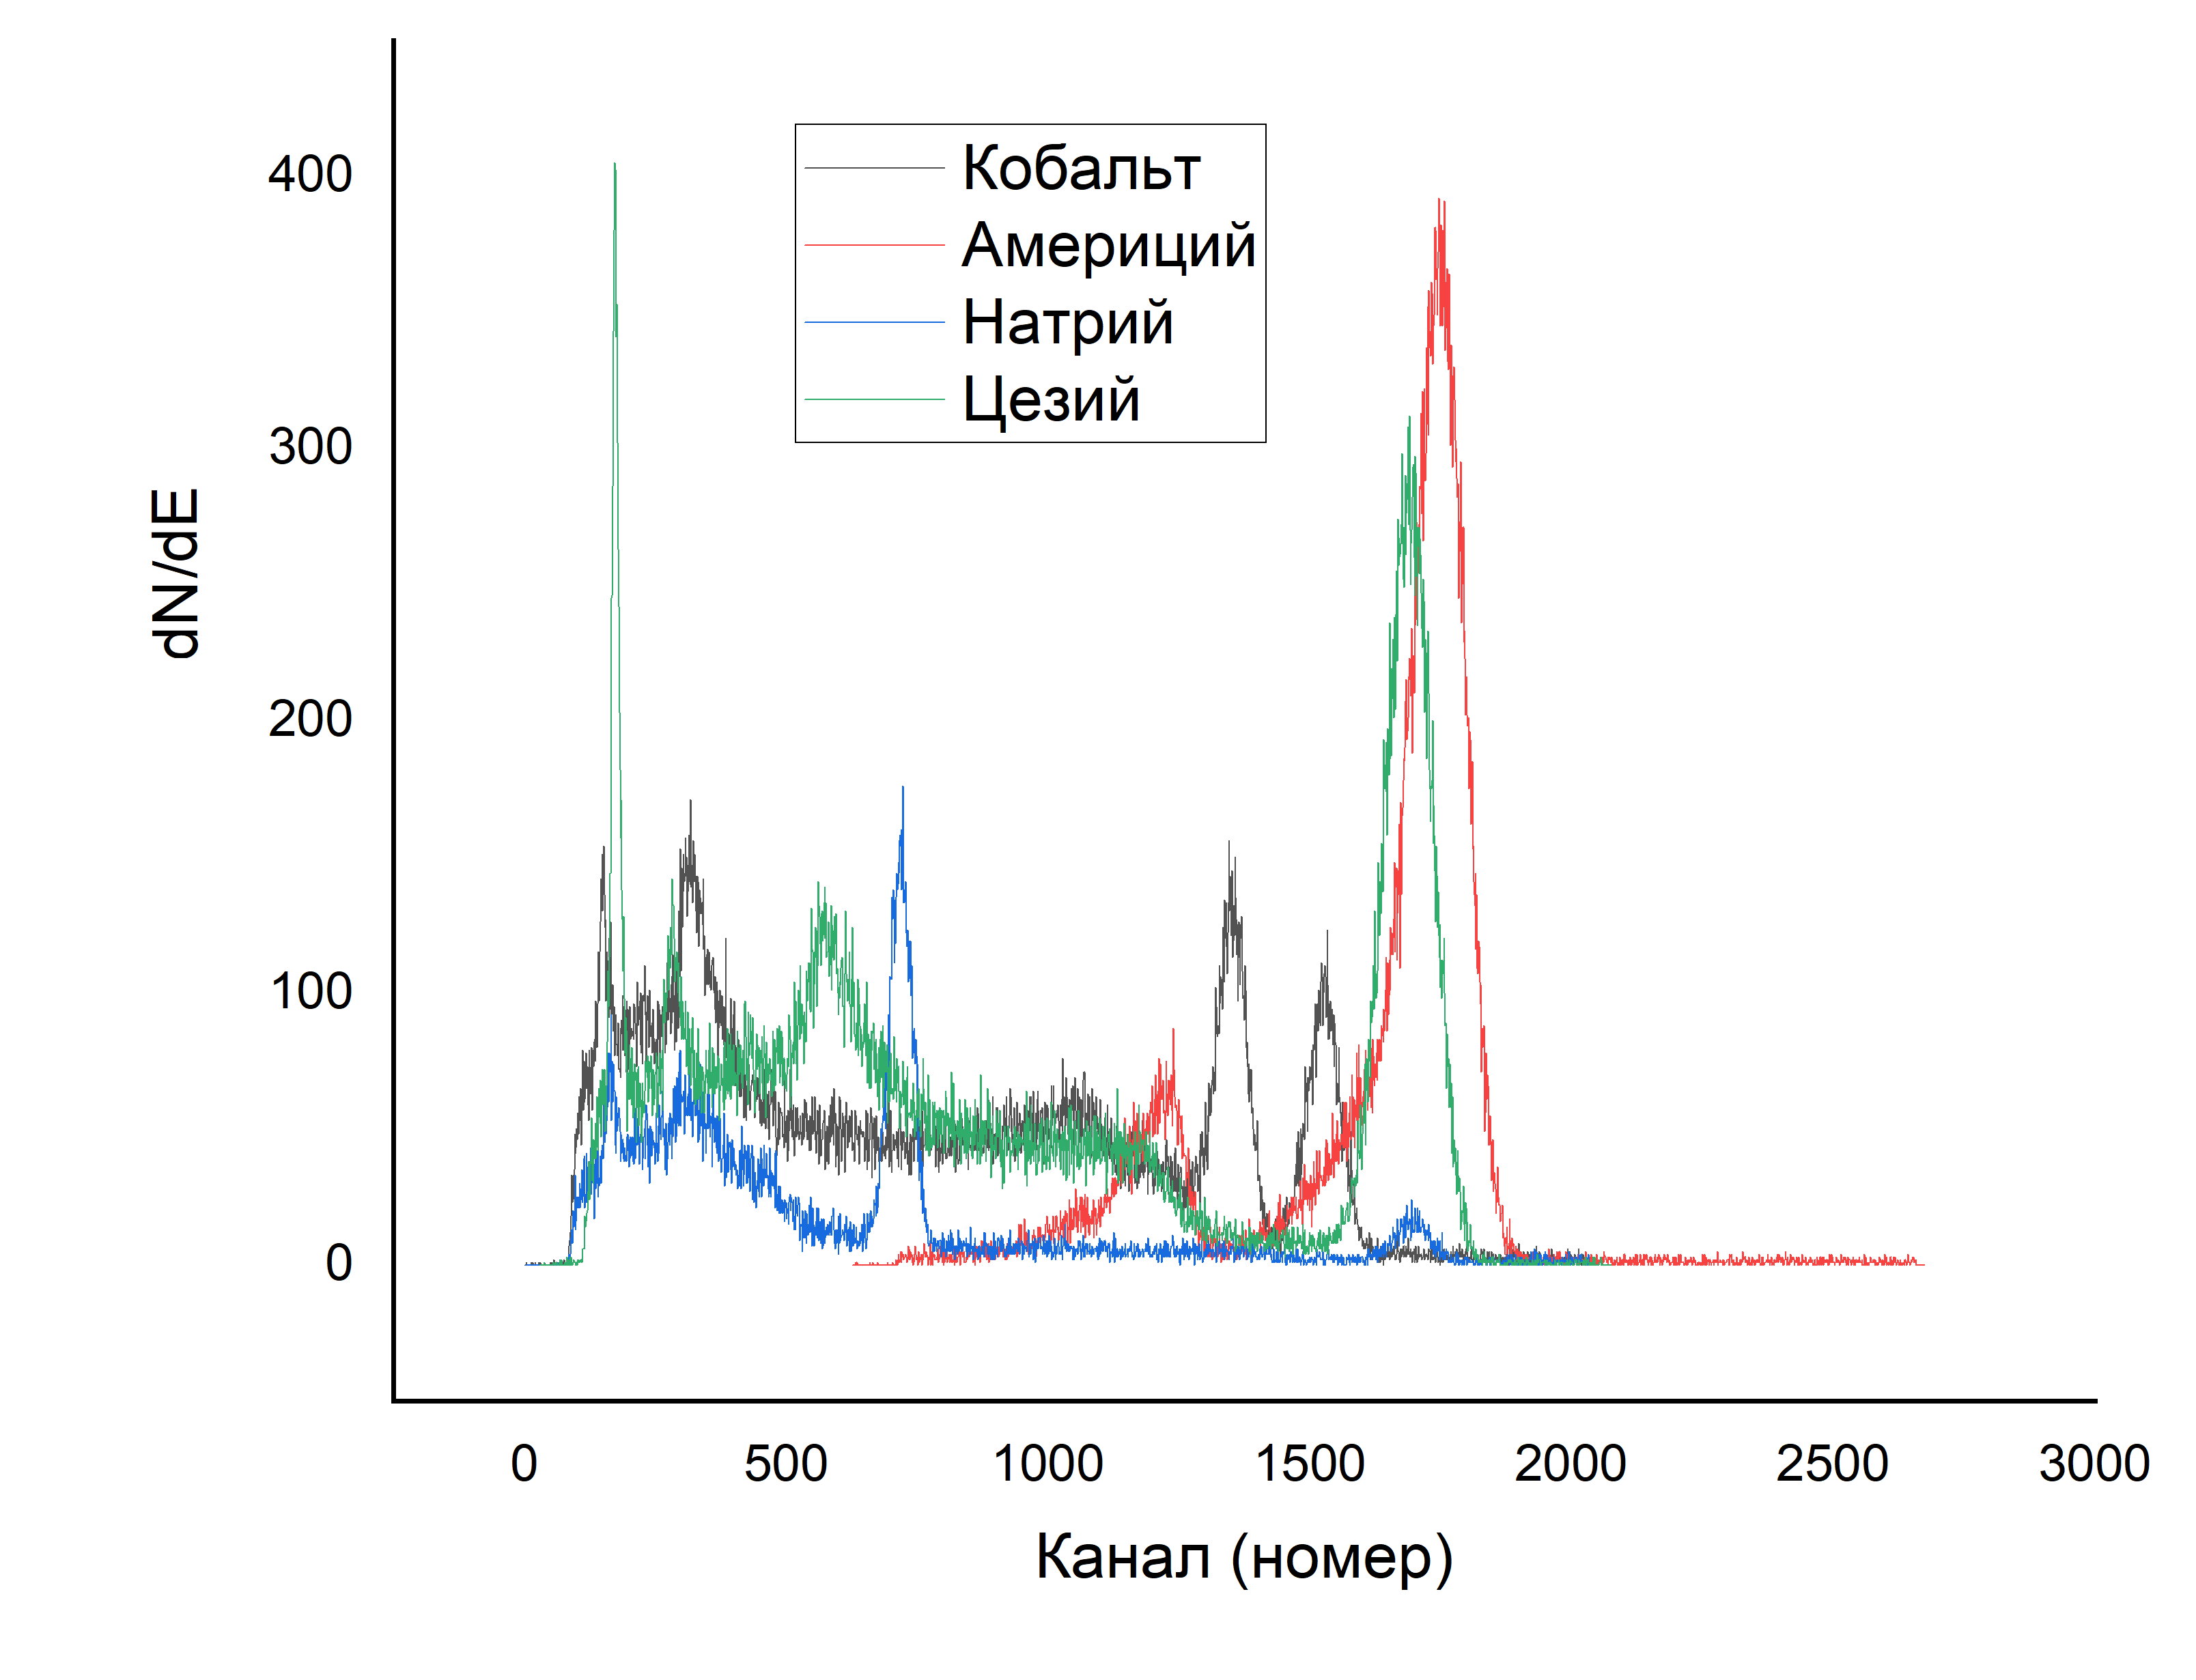
\includegraphics[scale=0.25]{3.png}
\end{figure*}


\begin{figure*}[]
	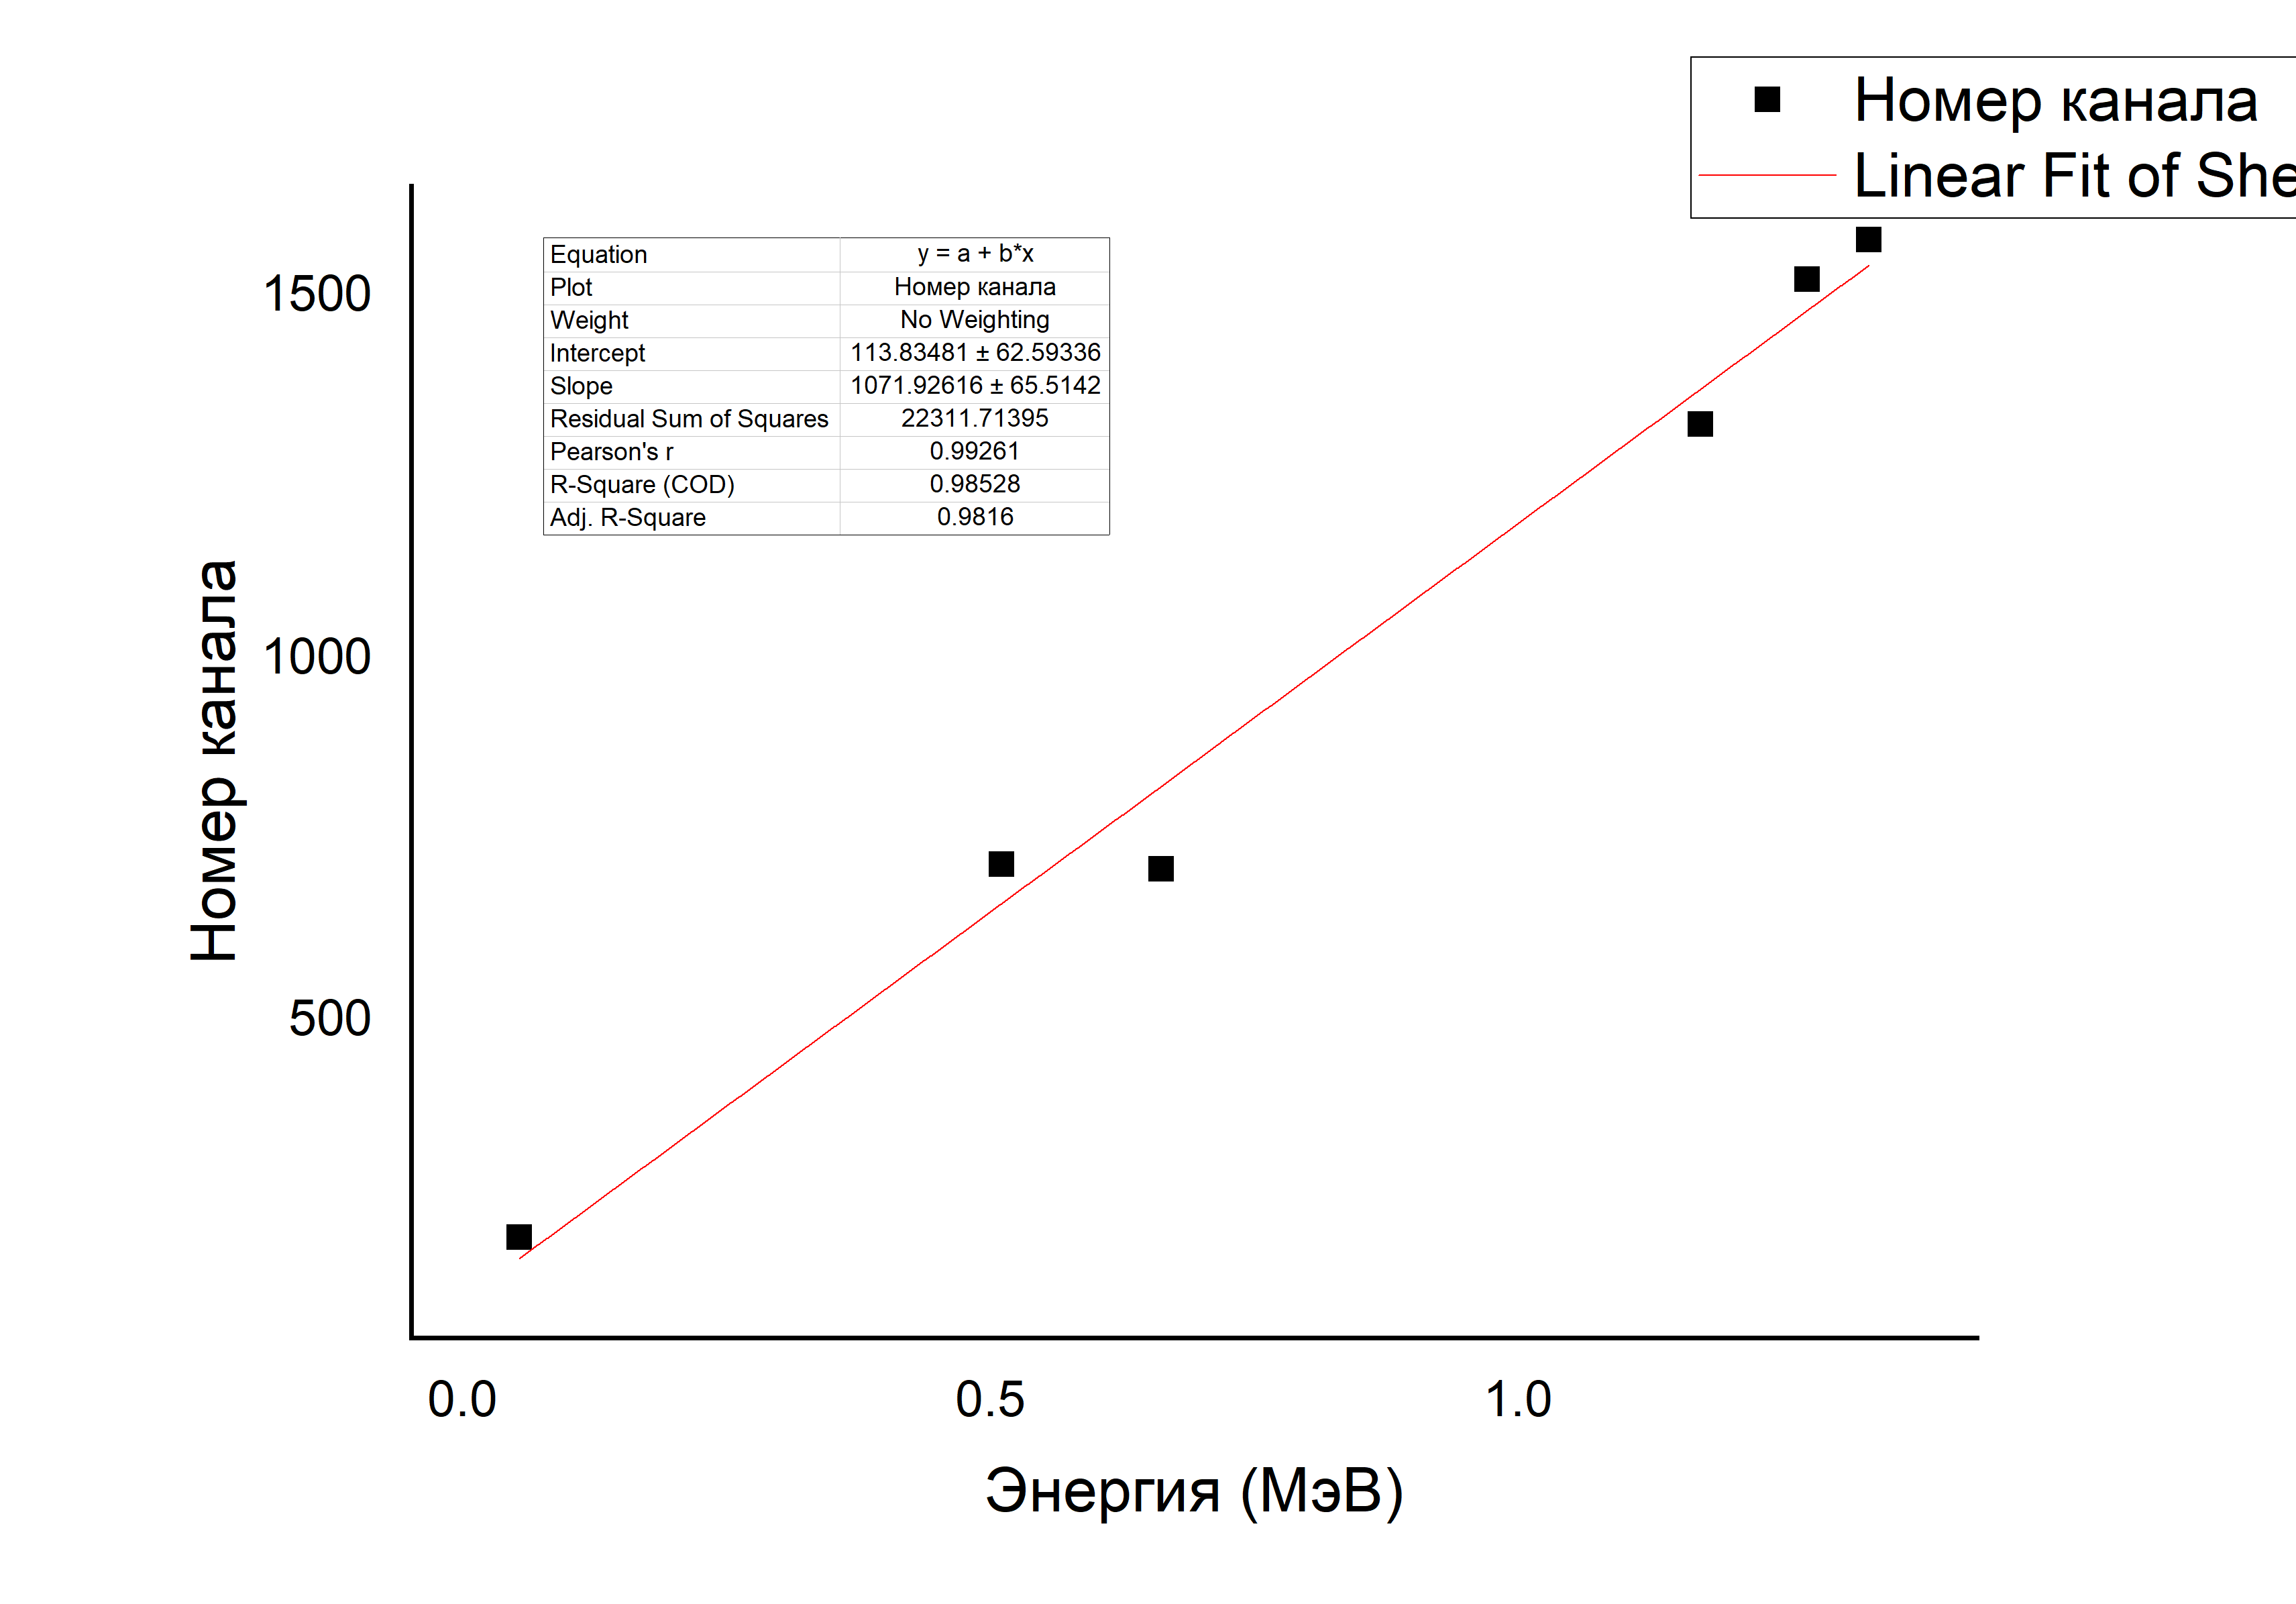
\includegraphics[scale=0.5]{4.png}
\end{figure*}



Для всех 4 образцов (полученный спектр Европия оказался слишком далеким от эталонного, потому был исключен из рассмотрения) получим следующую таблицу.

\begin{table}[]
	\begin{tabular}{|c|l|l|l|l|l|}
		\hline
		\multicolumn{1}{|l|}{Источник} & $N_i$  & $\Delta N_i$ & $E_i$, МэВ & $\Delta E_i$, МэВ & $R_i$     \\ \hline
		\multirow{2}{*}{Co-60}         & 1323  & 63.5                       & 1.1732    & 0.059235075                     & 0.05049  \\ \cline{2-6} 
		& 1578  & 72.4                       & 1.3325    & 0.067537313                     & 0.050685 \\ \hline
		\multirow{2}{*}{Na-22}         & 715.5 & 55.5                       & 0.511     & 0.051772388                     & 0.101316 \\ \cline{2-6} 
		& 1523  & 77.8                       & 1.274     & 0.072574627                     & 0.056966 \\ \hline
		Ce-137                         & 709   & 97.6                       & 0.6617    & 0.091044776                     & 0.137592 \\ \hline
		Am-241                         & 201   & 114                        & 0.054     & 0.106343284                     & 1.96932  \\ \hline
	\end{tabular}
\end{table}

Для всех данных, кроме Америция, проверим линейность зависимости $R^2 = f(1/E)$

\begin{figure*}[h!]
	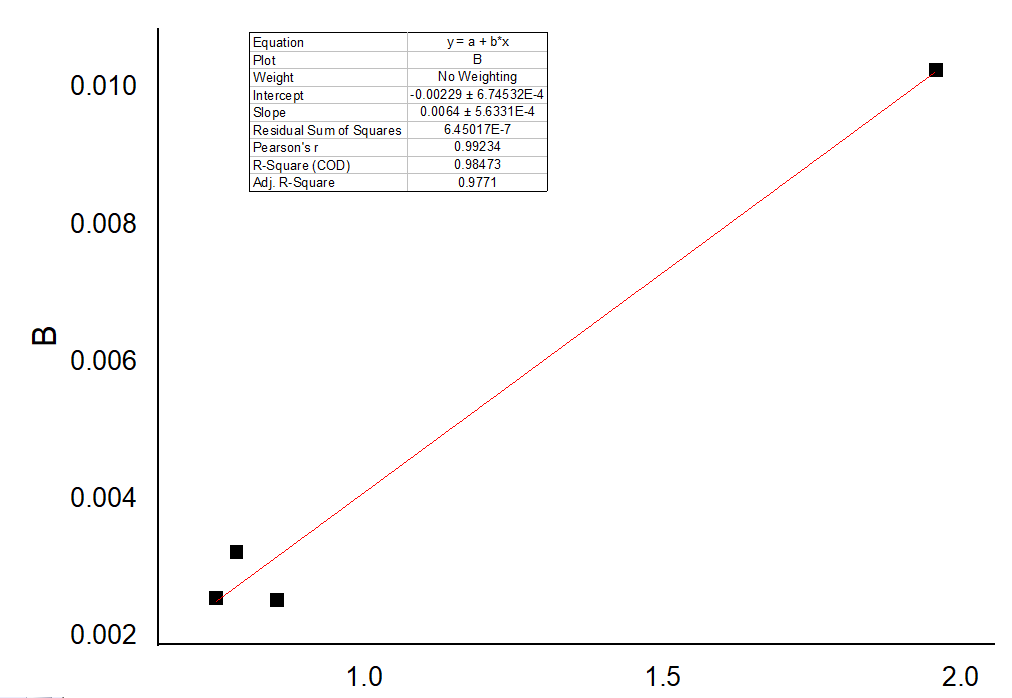
\includegraphics[scale=0.5]{5.png}
\end{figure*}
 Из графика можно заключить, что пик характеристического излучения свинца соответствует энергии примерно $300$ КэВ.
 
 Построим график энергий комптоновского края, одна из которых измеряется экспериментально по графику, другая - вычисляемая по формуле:
 
 \begin{equation}
 E_{max} = \frac{\eta \omega}{1 + \frac{mc^2}{2\eta \omega}}
 \end{equation}
 
 Однако этот подъем сглаживается за счет многократного рассеяния фотонов и конечного энергетического разрешения спектрометра, поэтому будем рассматривать канал пика, как середину снижения после пика.Поэтому погрешность измерения эксперемантального комптоновского края равна половине снижения, то есть расстояние от пика до низины по оси абцисс по полам. Так можно сравнить эксперементальную и расчетную комптоновские края.
 
 \begin{figure}[h!]
 	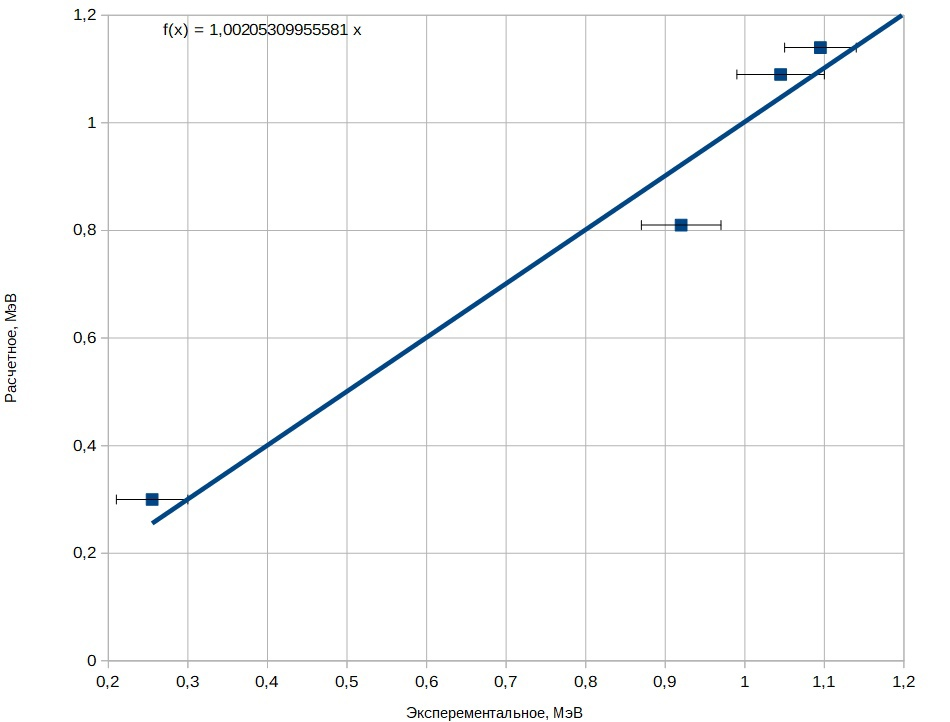
\includegraphics[scale=0.4]{6.jpg}
 \end{figure}
 
 Построим график зависимости энергии пика обратного рассеяния от
 энергии пика полного поглащения .Пик обратного рассеяния вычисляется по формуле:
 
 \begin{equation}
 E_{obr} = \frac{E}{1 + \frac{2E}{mc^2}}
 \end{equation}
 
 \begin{figure}[h!]
 	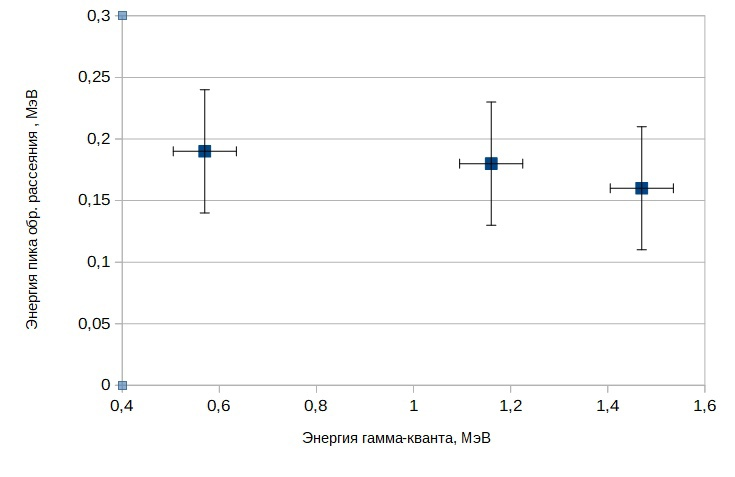
\includegraphics[scale=0.5]{7.jpg}
 \end{figure}
 

\section{Заключение.}

1) Для всех образцов, кроме Европия, получены спектральные картины, близкие к эталонным.

2) Проверена зависимость разрешающей способности от энергии.

3) Построены графики график энергий комптоновского края и зависимости энергии пика обратного рассеяния от энергии пика полного поглащения.
\end{document}
%
% ****** End of file apssamp.tex ******
